\documentclass{standalone}
\usepackage{tikz}
\usetikzlibrary{patterns, positioning}


\begin{document}
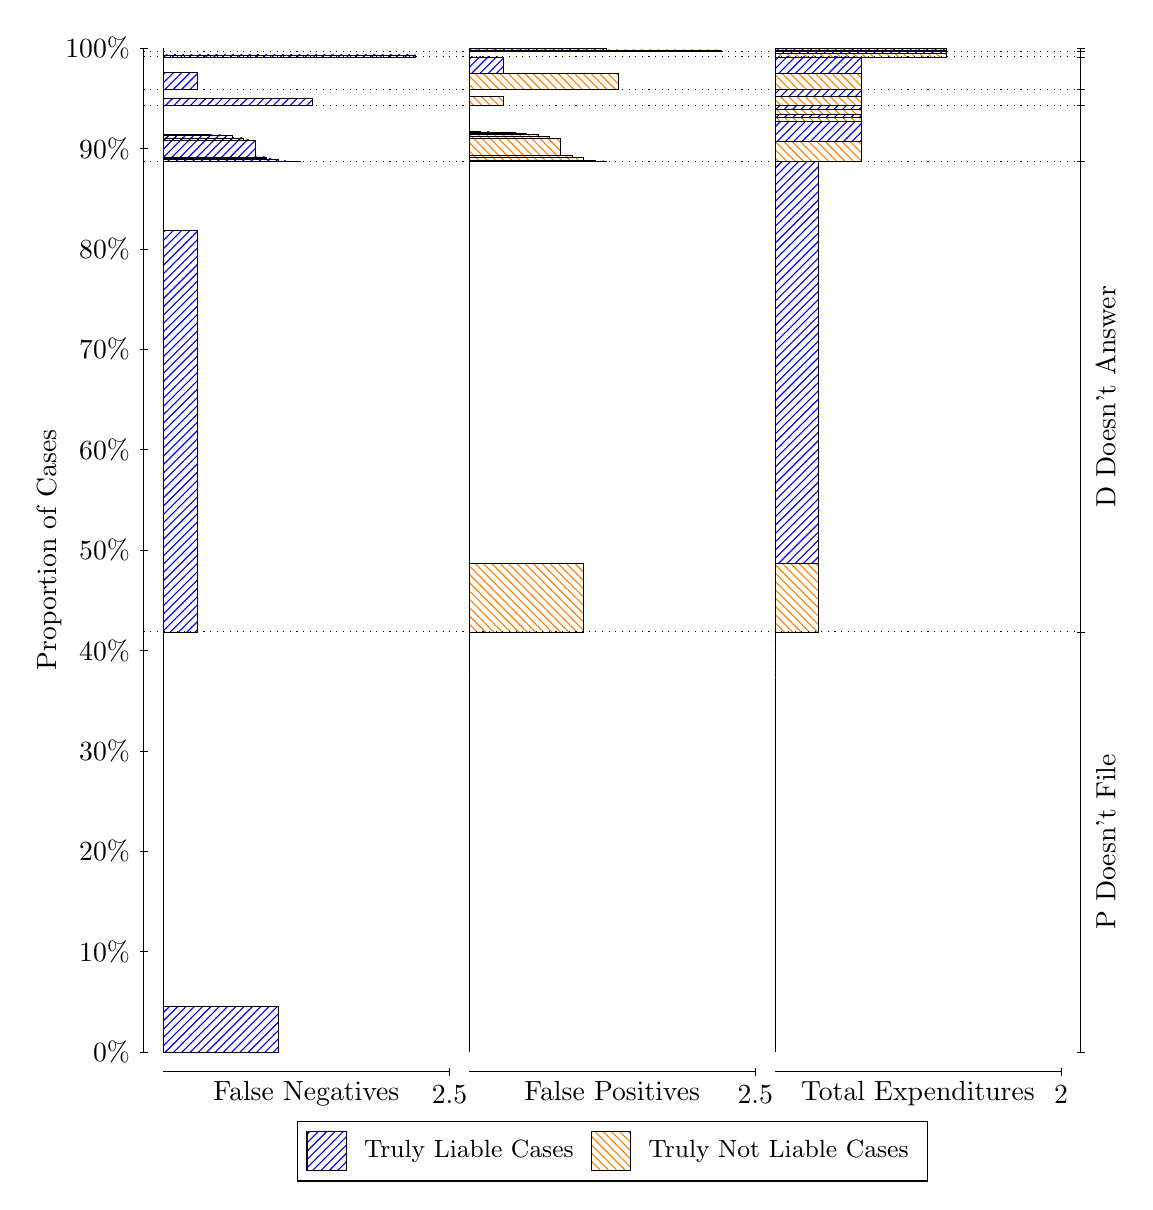
\begin{tikzpicture}
\draw[black, very thin] (1.5,1.75) -- (1.5,14.5);
\node[rotate=90, text=black, anchor=center] at (0.3, 8.125) {Proportion of Cases};
\draw[black, very thin] (1.45,1.75) -- (1.55,1.75);
\node[text=black, anchor=east] at (1.45, 1.75) {0\%};
\draw[black, very thin] (1.45,3.025) -- (1.55,3.025);
\node[text=black, anchor=east] at (1.45, 3.025) {10\%};
\draw[black, very thin] (1.45,4.3) -- (1.55,4.3);
\node[text=black, anchor=east] at (1.45, 4.3) {20\%};
\draw[black, very thin] (1.45,5.575) -- (1.55,5.575);
\node[text=black, anchor=east] at (1.45, 5.575) {30\%};
\draw[black, very thin] (1.45,6.85) -- (1.55,6.85);
\node[text=black, anchor=east] at (1.45, 6.85) {40\%};
\draw[black, very thin] (1.45,8.125) -- (1.55,8.125);
\node[text=black, anchor=east] at (1.45, 8.125) {50\%};
\draw[black, very thin] (1.45,9.4) -- (1.55,9.4);
\node[text=black, anchor=east] at (1.45, 9.4) {60\%};
\draw[black, very thin] (1.45,10.675) -- (1.55,10.675);
\node[text=black, anchor=east] at (1.45, 10.675) {70\%};
\draw[black, very thin] (1.45,11.95) -- (1.55,11.95);
\node[text=black, anchor=east] at (1.45, 11.95) {80\%};
\draw[black, very thin] (1.45,13.225) -- (1.55,13.225);
\node[text=black, anchor=east] at (1.45, 13.225) {90\%};
\draw[black, very thin] (1.45,14.5) -- (1.55,14.5);
\node[text=black, anchor=east] at (1.45, 14.5) {100\%};

\draw[black, very thin] (13.4,1.75) -- (13.4,14.5);
\draw[black, very thin] (13.35,1.75) -- (13.45,1.75);
\node[anchor=west] at (13.35, 1.75) {};
\draw[black, very thin] (13.35,7.0853) -- (13.45,7.0853);
\node[anchor=west] at (13.35, 7.0853) {};
\draw[black, very thin] (13.35,13.057) -- (13.45,13.057);
\node[anchor=west] at (13.35, 13.057) {};
\draw[black, very thin] (13.35,13.775) -- (13.45,13.775);
\node[anchor=west] at (13.35, 13.775) {};
\draw[black, very thin] (13.35,13.975) -- (13.45,13.975);
\node[anchor=west] at (13.35, 13.975) {};
\draw[black, very thin] (13.35,14.388) -- (13.45,14.388);
\node[anchor=west] at (13.35, 14.388) {};
\draw[black, very thin] (13.35,14.455) -- (13.45,14.455);
\node[anchor=west] at (13.35, 14.455) {};
\draw[black, very thin] (13.35,14.5) -- (13.45,14.5);
\node[anchor=west] at (13.35, 14.5) {};

\draw[black, very thin, pattern color=blue, pattern=north east lines] (1.75,1.75) rectangle (3.2033,2.3285);
\draw[black, very thin, pattern color=orange, pattern=north west lines] (1.75,2.3285) rectangle (1.75,7.0853);
\draw[black, very thin, pattern color=blue, pattern=north east lines] (1.75,7.0853) rectangle (2.186,12.186);
\draw[black, very thin, pattern color=orange, pattern=north west lines] (1.75,12.186) rectangle (1.75,13.057);
\draw[black, very thin, pattern color=blue, pattern=north east lines] (1.75,13.057) rectangle (3.494,13.062);
\draw[black, very thin, pattern color=blue, pattern=north east lines] (1.75,13.062) rectangle (3.3487,13.066);
\draw[black, very thin, pattern color=blue, pattern=north east lines] (1.75,13.066) rectangle (3.2033,13.093);
\draw[black, very thin, pattern color=blue, pattern=north east lines] (1.75,13.093) rectangle (3.058,13.095);
\draw[black, very thin, pattern color=blue, pattern=north east lines] (1.75,13.095) rectangle (3.058,13.118);
\draw[black, very thin, pattern color=blue, pattern=north east lines] (1.75,13.118) rectangle (2.9127,13.334);
\draw[black, very thin, pattern color=blue, pattern=north east lines] (1.75,13.334) rectangle (2.7673,13.358);
\draw[black, very thin, pattern color=blue, pattern=north east lines] (1.75,13.358) rectangle (2.622,13.389);
\draw[black, very thin, pattern color=blue, pattern=north east lines] (1.75,13.389) rectangle (2.4767,13.397);
\draw[black, very thin, pattern color=blue, pattern=north east lines] (1.75,13.397) rectangle (2.3313,13.408);
\draw[black, very thin, pattern color=orange, pattern=north west lines] (1.75,13.408) rectangle (1.75,13.775);
\draw[black, very thin, pattern color=blue, pattern=north east lines] (1.75,13.775) rectangle (3.6393,13.86);
\draw[black, very thin, pattern color=orange, pattern=north west lines] (1.75,13.86) rectangle (1.75,13.975);
\draw[black, very thin, pattern color=blue, pattern=north east lines] (1.75,13.975) rectangle (2.186,14.187);
\draw[black, very thin, pattern color=orange, pattern=north west lines] (1.75,14.187) rectangle (1.75,14.388);
\draw[black, very thin, pattern color=blue, pattern=north east lines] (1.75,14.388) rectangle (4.9473,14.412);
\draw[black, very thin, pattern color=orange, pattern=north west lines] (1.75,14.412) rectangle (1.75,14.455);
\draw[black, very thin, pattern color=orange, pattern=north west lines] (1.75,14.455) rectangle (1.75,14.475);
\draw[black, very thin, pattern color=blue, pattern=north east lines] (1.75,14.475) rectangle (1.75,14.5);
\draw[black, very thin, pattern color=orange, pattern=north west lines] (5.6333,1.75) rectangle (5.6333,6.5068);
\draw[black, very thin, pattern color=blue, pattern=north east lines] (5.6333,6.5068) rectangle (5.6333,7.0853);
\draw[black, very thin, pattern color=orange, pattern=north west lines] (5.6333,7.0853) rectangle (7.0867,7.9567);
\draw[black, very thin, pattern color=blue, pattern=north east lines] (5.6333,7.9567) rectangle (5.6333,13.057);
\draw[black, very thin, pattern color=orange, pattern=north west lines] (5.6333,13.057) rectangle (7.3773,13.067);
\draw[black, very thin, pattern color=orange, pattern=north west lines] (5.6333,13.067) rectangle (7.232,13.076);
\draw[black, very thin, pattern color=orange, pattern=north west lines] (5.6333,13.076) rectangle (7.0867,13.108);
\draw[black, very thin, pattern color=orange, pattern=north west lines] (5.6333,13.108) rectangle (6.9413,13.133);
\draw[black, very thin, pattern color=orange, pattern=north west lines] (5.6333,13.133) rectangle (6.796,13.352);
\draw[black, very thin, pattern color=orange, pattern=north west lines] (5.6333,13.352) rectangle (6.6507,13.377);
\draw[black, very thin, pattern color=orange, pattern=north west lines] (5.6333,13.377) rectangle (6.5053,13.408);
\draw[black, very thin, pattern color=orange, pattern=north west lines] (5.6333,13.408) rectangle (6.36,13.415);
\draw[black, very thin, pattern color=orange, pattern=north west lines] (5.6333,13.415) rectangle (6.2147,13.424);
\draw[black, very thin, pattern color=blue, pattern=north east lines] (5.6333,13.424) rectangle (5.924,13.435);
\draw[black, very thin, pattern color=blue, pattern=north east lines] (5.6333,13.435) rectangle (5.7787,13.443);
\draw[black, very thin, pattern color=blue, pattern=north east lines] (5.6333,13.443) rectangle (5.6333,13.775);
\draw[black, very thin, pattern color=orange, pattern=north west lines] (5.6333,13.775) rectangle (6.0693,13.89);
\draw[black, very thin, pattern color=blue, pattern=north east lines] (5.6333,13.89) rectangle (5.6333,13.975);
\draw[black, very thin, pattern color=orange, pattern=north west lines] (5.6333,13.975) rectangle (7.5227,14.176);
\draw[black, very thin, pattern color=blue, pattern=north east lines] (5.6333,14.176) rectangle (6.0693,14.388);
\draw[black, very thin, pattern color=orange, pattern=north west lines] (5.6333,14.388) rectangle (5.6333,14.43);
\draw[black, very thin, pattern color=blue, pattern=north east lines] (5.6333,14.43) rectangle (5.6333,14.455);
\draw[black, very thin, pattern color=orange, pattern=north west lines] (5.6333,14.455) rectangle (8.8307,14.475);
\draw[black, very thin, pattern color=blue, pattern=north east lines] (5.6333,14.475) rectangle (7.3773,14.5);
\draw[black, very thin, pattern color=orange, pattern=north west lines] (9.5167,1.75) rectangle (9.5167,6.5068);
\draw[black, very thin, pattern color=blue, pattern=north east lines] (9.5167,6.5068) rectangle (9.5167,7.0853);
\draw[black, very thin, pattern color=orange, pattern=north west lines] (9.5167,7.0853) rectangle (10.062,7.9567);
\draw[black, very thin, pattern color=blue, pattern=north east lines] (9.5167,7.9567) rectangle (10.062,13.057);
\draw[black, very thin, pattern color=orange, pattern=north west lines] (9.5167,13.057) rectangle (10.607,13.316);
\draw[black, very thin, pattern color=blue, pattern=north east lines] (9.5167,13.316) rectangle (10.607,13.571);
\draw[black, very thin, pattern color=orange, pattern=north west lines] (9.5167,13.571) rectangle (10.607,13.621);
\draw[black, very thin, pattern color=blue, pattern=north east lines] (9.5167,13.621) rectangle (10.607,13.659);
\draw[black, very thin, pattern color=orange, pattern=north west lines] (9.5167,13.659) rectangle (10.607,13.717);
\draw[black, very thin, pattern color=blue, pattern=north east lines] (9.5167,13.717) rectangle (10.607,13.775);
\draw[black, very thin, pattern color=orange, pattern=north west lines] (9.5167,13.775) rectangle (10.607,13.89);
\draw[black, very thin, pattern color=blue, pattern=north east lines] (9.5167,13.89) rectangle (10.607,13.975);
\draw[black, very thin, pattern color=orange, pattern=north west lines] (9.5167,13.975) rectangle (10.607,14.176);
\draw[black, very thin, pattern color=blue, pattern=north east lines] (9.5167,14.176) rectangle (10.607,14.388);
\draw[black, very thin, pattern color=orange, pattern=north west lines] (9.5167,14.388) rectangle (11.697,14.43);
\draw[black, very thin, pattern color=blue, pattern=north east lines] (9.5167,14.43) rectangle (11.697,14.455);
\draw[black, very thin, pattern color=orange, pattern=north west lines] (9.5167,14.455) rectangle (11.697,14.475);
\draw[black, very thin, pattern color=blue, pattern=north east lines] (9.5167,14.475) rectangle (11.697,14.5);
\draw[black, dotted] (1.5,7.0853) -- (13.4,7.0853);
\draw[black, dotted] (1.5,13.057) -- (13.4,13.057);
\draw[black, dotted] (1.5,13.775) -- (13.4,13.775);
\draw[black, dotted] (1.5,13.975) -- (13.4,13.975);
\draw[black, dotted] (1.5,14.388) -- (13.4,14.388);
\draw[black, dotted] (1.5,14.455) -- (13.4,14.455);
\draw[black, very thin] (1.75,1.5) -- (5.3833,1.5);
\node[text=black, anchor=north] at (3.5667, 1.5) {False Negatives};
\draw[black, very thin] (5.3833,1.45) -- (5.3833,1.55);
\node[text=black, anchor=north] at (5.3833, 1.45) {2.5};

\draw[black, very thin] (5.6333,1.5) -- (9.2667,1.5);
\node[text=black, anchor=north] at (7.45, 1.5) {False Positives};
\draw[black, very thin] (9.2667,1.45) -- (9.2667,1.55);
\node[text=black, anchor=north] at (9.2667, 1.45) {2.5};

\draw[black, very thin] (9.5167,1.5) -- (13.15,1.5);
\node[text=black, anchor=north] at (11.333, 1.5) {Total Expenditures};
\draw[black, very thin] (13.15,1.45) -- (13.15,1.55);
\node[text=black, anchor=north] at (13.15, 1.45) {2};

\node[text=black, centered, rotate=90] at (13.72, 4.4177) {P Doesn't File};
\node[text=black, centered, rotate=90] at (13.72, 10.071) {D Doesn't Answer};






\draw (7.449999999999999,1.5) node[draw=none] (baseCoordinate) {};
\begin{scope}[align=center]
        \matrix[scale=0.5, draw=black, below=0.5cm of baseCoordinate, nodes={draw}, column sep=0.1cm]{
            \node[rectangle, draw, minimum width=0.5cm, minimum height=0.5cm, pattern color=blue, pattern=north east lines] {}; &
            \node[draw=none, font=\small, text=black] (B) {Truly Liable Cases}; &
            \node[rectangle, draw, minimum width=0.5cm, minimum height=0.5cm, pattern color=orange, pattern=north west lines] {}; &
            \node[draw=none, font=\small, text=black] (B) {Truly Not Liable Cases}; \\
            };
\end{scope}

\end{tikzpicture}
\end{document}